\documentclass[a4paper,10pt]{article}
\usepackage{My_math_package}



\title{MATH620 - Algebraic Number Theory}
\author{Haoran Li}
\date{2018 Fall}

\makeindex[columns=2, title=Index, intoc] % Create the index

\begin{document}\sloppy % reduce overlong words

% Maketitle
\begin{titlepage}
\begin{center}
\vspace*{1cm}
\LARGE
\textbf{MATH620 - Algebraic Number Theory} \\
\vspace{2cm}
\begin{center}
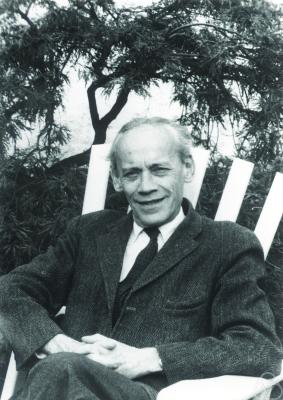
\includegraphics[width=0.5\textwidth]{Pictures/Emil_Artin.jpg}
\end{center}
\vspace{2cm}
\normalsize
Taught by \texttt{Niranjan Ramachandran} \\
Notes taken by \texttt{Haoran Li} \\
2020 Spring \\
\vspace{2cm}
Department of Mathematics\\
University of Maryland\\
\end{center}
\end{titlepage}

\tableofcontents
\newpage

\section{Disciminant}
\subfile{Discriminant.tex}
\newpage

\section{Minkowski's theorem}
\subfile{Minkowski's_theorem.tex}
\newpage

\section{Dirichlet's unit theorem}
\subfile{Dirichlet's_unit_theorem.tex}
\newpage

\section{Discrete valuation domain}
\subfile{Discrete_valuation_domain.tex}
\newpage

\section{Ramification}
\subfile{Ramification.tex}
\newpage

\begin{thebibliography}{}



\end{thebibliography}

\printindex
\newpage

\end{document}